\documentclass{article}
\newcommand{\BEAS}{\begin{eqnarray*}}
\newcommand{\EEAS}{\end{eqnarray*}}
\newcommand{\BEQ}{\begin{equation}}
\newcommand{\EEQ}{\end{equation}}
\newcommand{\BIT}{\begin{itemize}}
\newcommand{\EIT}{\end{itemize}}

\newcommand{\eg}{{\it e.g.\ }}
\newcommand{\ie}{{\it i.e.\ }}

\newcommand{\ones}{\mathbf 1}
\newcommand{\zeros}{\mathbf 0}
\newcommand{\reals}{{\mbox{\bf R}}}
\newcommand{\integers}{{\mbox{\bf Z}}}
\newcommand{\symm}{{\mbox{\bf S}}}  % symmetric matrices

\newcommand{\nullspace}{{\mathcal N}}
\newcommand{\range}{{\mathcal R}}
\newcommand{\Rank}{\mathop{\bf Rank}}
\newcommand{\Tr}{\mathop{\bf Tr}}

\newcommand{\sign}[1]{\mathop{\textrm{sgn}}(#1)}
\newcommand{\lambdamax}{{\lambda_{\rm max}}}
\newcommand{\lambdamin}{\lambda_{\rm min}}

\newcommand{\EE}{\mathop{\textrm{E}}}
\newcommand{\Cov}{\mathop{\textrm{Cov}}}
\newcommand{\Prob}{\mathop{\bf Prob}}
\newcommand{\Co}{{\mathop {\bf Co}}} % convex hull
\newcommand{\dist}{\mathop{\bf dist{}}}
\newcommand{\argmin}{\mathop{\rm argmin}}
\newcommand{\argmax}{\mathop{\rm argmax}}
\newcommand{\epi}{\mathop{\bf epi}} % epigraph
\newcommand{\Vol}{\mathop{\bf vol}}
\newcommand{\dom}{\mathop{\bf dom}} % domain
\newcommand{\intr}{\mathop{\bf int}}


\newcommand{\nrm}[1]{\left\lVert#1\right\rVert}
\newcommand{\nrmo}[1]{\left\lVert#1\right\rVert_1}
\newcommand{\nrmt}[1]{\left\lVert#1\right\rVert_2}
\newcommand{\nrmnn}[1]{\left\lVert#1\right\rVert_{*}}
\newcommand{\nrmf}[1]{\left\lVert#1\right\rVert_F}

\newcommand{\myexp}[1]{\mathop{\rm exp}\left\{#1\right\}}
\newcommand{\mylog}[1]{\mathop{\rm log}\left\{#1\right\}}
\newcommand{\questions}{\begin{frame}Questions?\end{frame}}
\newcommand{\LL}{\textrm{LL}}
\newcommand{\KL}{\textrm{KL}}
\newcommand{\HH}{\textrm{H}}
\newcommand{\GG}{\textrm{G}}

\newcommand{\Bound}{\textrm{B}}
\newcommand{\bb}{\mathbf{b}}
\newcommand{\aaa}{\mathbf{a}}
\newcommand{\BB}{\mathbf{B}}
\newcommand{\AAA}{\mathbf{A}}
\newcommand{\CC}{\mathbf{C}}
\newcommand{\cc}{\mathbf{c}}
\newcommand{\mm}{\mathbf{m}}
\newcommand{\MM}{\mathbf{M}}
\newcommand{\nn}{\mathrm{\bf neighbors}}
\newcommand{\pa}[1]{{\textrm{\bf pa}}\left(#1\right)}
\newcommand{\pre}[2]{\mathop{\textrm{\bf pnp}}_{#1}\left(#2\right)}
\newcommand{\logsum}{\textrm{logsum}}

\newcommand{\tth}{{\textrm{th}}}
\newcommand{\xx}{\mathbf{x}}
\newcommand{\mmu}{\mathbf{\mu}}
\newcommand{\yy}{\mathbf{y}}
\newcommand{\zz}{\mathbf{z}}
\newcommand{\dd}{\mathbf{d}}
\newcommand{\new}{\textrm{new}}
\newcommand{\old}{\textrm{old}}
\newcommand{\fpr}{\textrm{FPR}}
\newcommand{\tpr}{\textrm{TPR}}
\newcommand{\auc}{\textrm{AUC}}
\newcommand{\yyi}{\yy_i}
\newcommand{\xxi}{\xx_i}
\newcommand{\vvec}[2]{\left[ \begin{array}{c} \mathbf{#1}\\ \mathbf{#2} \end{array}\right]}
\newcommand{\mmat}[4]{\left[ \begin{array}{cc} \mathbf{#1}&\mathbf{#2}\\ \mathbf{#3}&\mathbf{#4} \end{array}\right]}
\newcommand{\xyvec}{\left[ \begin{array}{c} \xx\\\yy \end{array} \right]}
\newcommand{\xyvecc}{\left[ \begin{array}{c} x^1\\y^1 \end{array} \right]}
\newcommand{\eye}{   \left[ \begin{array}{cc} 1 & 0 \\ 0 & 1 \end{array}\right]}
\newcommand{\bket}[2]{\left\langle#1,#2\right\rangle}
\newcommand{\bbket}[2]{\left\llangle#1,#2\right\rrangle}
\newcommand{\redq}{\textcolor{red}{q}}
\newcommand{\blup}{\textcolor{blue}{p}}
\newcommand{\BIEA}{\begin{IEEEeqnarray*}}
\newcommand{\EIEA}{\end{IEEEeqnarray*}}
\newcommand{\BIEAN}{\begin{IEEEeqnarray}}
\newcommand{\EIEAN}{\end{IEEEeqnarray}}
\newcommand{\pmin}{\mathop{\textrm{minimize}}}
\newcommand{\psubjto}{\textrm{subject to}}
\newcommand{\WW}{\mathbf{W}}
\newcommand{\ww}{\mathbf{w}}
\newcommand{\YY}{\mathbf{Y}}
\newcommand{\XX}{\mathbf{X}}
\newcommand{\UU}{\mathbf{U}}
\newcommand{\uu}{\mathbf{u}}
\newcommand{\VV}{\mathbf{V}}
\newcommand{\vv}{\mathbf{v}}
\newcommand{\PP}{\mathbf{P}}
\newcommand{\pp}{\mathbf{p}}
\newcommand{\rr}{\mathbf{r}}
\newcommand{\RR}{\mathbf{R}}
\newcommand{\ee}{\mathbf{e}}
\newcommand{\II}{\mathbf{I}}
\newcommand{\DD}{\mathbf{D}}

\newcommand{\aalpha}{{\boldsymbol\alpha}}
\newcommand{\llambda}{{\boldsymbol\lambda}}
\newcommand{\ddelta}{{\boldsymbol\delta}}
\newcommand{\otherwise}{\textrm{otherwise}}
\newcommand{\answer}{\fbox{\tt answer} }
\newcommand{\abs}[1]{\left| #1 \right|}

\newcounter{problemCtr}
\newcommand{\newproblem}[1]{\hrule\paragraph{Problem \theproblemCtr (#1)}\stepcounter{problemCtr}}


\newcounter{HW}

\usepackage{amsthm}
\usepackage{graphicx}
\usepackage{natbib}
\usepackage{algorithm}
\usepackage{algorithmic}
\usepackage{amsmath}
\usepackage{hyperref}
\usepackage{tikz}


\newtheorem{remark}{Remark}
\newtheorem{lemma}{Lemma}
\newtheorem{definition}{Definition}
\newtheorem{proposition}{Proposition}
\newtheorem{assumption}{Assumption}
\newtheorem{corollary}{Corollary}
\newtheorem{theorem}{Theorem}


\begin{document}
\author{Wile E. Coyote}
\setcounter{HW}{2}
\title{COMP  790-125, HW\theHW}
\maketitle


{ Deadline: 11/5/2015 11:59PM EST}

{ Submit \texttt{hw\theHW.pdf} by e-mail to \texttt{vjojic+comp790+hw\theHW@cs.unc.edu}



\noindent\rule{\textwidth}{3pt}

Read carefully and fill in the details. This homework is not meant to be difficult, rather it is meant
to establish flow of putting together a generative model, and developing an EM algorithm.


We will derive and an algorithm for motif discovery. 

We are given
\begin{itemize}
\item an alphabet $\mathcal{A}$
\item a dataset of sequences over the alphabet, each containing a subsequence conforming to a pattern.
\end{itemize}
The task of motif discovery is to uncover the pattern.


Here is a simple example of a motif discovery dataset
\begin{verbatim}
VCKMMOMMOMUDG
QGMOMMOMBIKYJ
JDXXGYVMOMMOM
NFYJKMOMMOMOA
KMOMMOMGMDCBB
\end{verbatim}
The motif here is \verb|MOMMOM|.

\vskip 5pt

Our approach is going to be to specify a probabilistic model that might have been used
to generate the dataset. Then we will train this model on the dataset to obtain parameters
describing the pattern. 


\newproblem{2pt}
We will propose a probabilistic model for motif sequences of length $L$.
Under this model, any sequence of length $L$ will have a non-zero probability.
However, a trained model ought to assign low probability to most sequences.

Our probabilistic model for a sequence generated from a motif will be given by
\[
p(\xx|\theta) = \prod_{i=1}^L\prod_{a \in \mathcal{A}} \theta_{a,i}^{[x_i = a]}.
\]
where $\xx$ is a sequence, and $\theta$ are parameters describing a motif.
Note that $\theta$ is of size $A \times L$ where A is size of alphabet, and L is length of sequence.
We will assume that $\theta_{i,a} > 0$ and $\sum_a \theta_{i,a} = 1$. Hence, every column
of matrix $\theta$ is a categorical distribution.

\paragraph{Sampling categorical distribution} We will need to sample discrete distribution. So, we will
write code for this.

Implement inverse cdf sampling for a discrete distribution
\begin{verbatim}
function s = samplediscrete(ps,T)
cdf = cumsum( ... )
S = zeros(T,1);
for t=1:T
     r = rand(1,1);
     s(t) = find( ... , 1);
end
\end{verbatim}

\verb|find(vec,1)| finds first occurrence of a non-zero value in vector \verb|vec| and returns its index.


Check your code by 
\begin{verbatim}
ps = [0.1 0.3 0.6];
T = 1000;
data = samplediscrete(ps,1000);
f = [sum(data==1)/T sum(data==2)/T sum(data==3)/T]
\end{verbatim}
If you did everything right, vector of frequencies \verb|f| should be close to the vector of probabilities used
to draw the sample \verb|ps|. Something like
\begin{verbatim}
f =
    0.0940    0.3110    0.5950
\end{verbatim}

\paragraph{Generating a $\theta$ matrix} In order to play with synthetic data, we will need
to generate a $\theta$ matrix. You could do this by hand, but we can also generate it randomly.
We want a matrix that puts much of its probability mass on one or two of possible states. 

\begin{verbatim}
function theta = randomtheta(A,L)
theta = rand(A,L)
theta = theta.^10;
theta = theta./repmat(sum(theta),[A 1]);
\end{verbatim}

The code above raises entries to the $10^{\tth}$ power.
Play with different exponents and compare outputs of \verb|randomtheta|.
Explain what happens. \answer

\paragraph{Sampling sequences from the model}
We will write code to generate synthetic sequences from a motif model (specified by a $\theta$ matrix).

Recall that we represent sequences as binary matrices rather than strings.

Implement code that samples sequences given a motif.
\begin{verbatim}
function X = samplemotif(theta,T)
A = size(theta,1); % size of alphabet
L = size(theta,2); % length of motif
% does each column sum to 1
assert(all(abs(sum(theta,1) - 1.0)<1e-6))
% are all probabilities greater than 0
assert(all(theta(:)>0))
X = zeros(A,L,T);
for t=1:T
    for i=1:L
        % drawn a single letter according to theta(:,i)
        letter = samplediscrete(...);
        X(letter,i,t) = 1;
    end
end
\end{verbatim}

Generate some motifs

\begin{verbatim}
A = 4; L = 5; T = 300;
groundtruththeta = randomtheta(A,L);
mymotifs = samplemotif(mytheta,T);
\end{verbatim}

Take a look at this data.


\paragraph{Computing probability of a sequence under motif model $\log p_f(\xx|\theta)$} 
We will denote probability of a motif sequence as $p_f$ where $f$ stands for foreground.

Our model tells us that probability of a sequence of length $L$ under motif model is 
\[
p_f(\xx|\theta) = \prod_{i=1}^L\prod_{a \in \mathcal{A}} \theta_{a,i}^{[x_i = a]}.
\]
Hence it's log is
\[
\log p_f(\xx|\theta) = ...
\]

Implement computation of the log probability, remember sequence input is a matrix of indicators not a string:
\begin{verbatim}
function lp = logpf(x,theta)
A = size(theta,1); % size of alphabet
L = size(theta,2); % length of motif
assert(size(x,1) == A && size(x,2) == L);
lp = sum( sum(... ) ) 
\end{verbatim}

\newproblem{2pt} In motif discovery task, we are provided with a set of sequences that contain
examples of the motif. We have not yet specified how to generate parts of the sequences that are 
outside of the motif. 

We will assume that parts of sequences that are not coming from a motif are generated from the alphabet
with uniform probability for each letter.
\[
p_b(x_i = a) = \frac{1}{|\mathcal{A}|}, \forall a \in \mathcal{A}
\]

Sometimes this is called a background model. The motif can be thought of as foreground.
Note that we are using $p_b$ to be able to distinguish foreground $p(\xx|\theta)$ and background model $p_b(\xx)$


\paragraph{Putting together motif and background models}
We wish to generate full sequences that contain the motif and the rest of the letters are just noise.
To do so, we need to decide where in the sequence the motif will occur. We will introduce a latent variable, $h$, that
stores offset at which the motif starts.  If a sequence is of length $N$, then $h \in  \{1,\dots,N-L+1\}$.
Why $N-L+1$? \answer

Since $h$ is a random variable we need to specify a prior distribution for it. 
We do not have any special information about where the motifs are likely to occur so we choose uniform
\[
p(h = i) = \frac{1}{N-L+1}.
\]

Let's write out joint probability of a sequence $\yy$ and an offset $h$:
\[
p(\xx,h|\theta) = \underbrace{p(h)}_A \underbrace{\left[\prod_{i=1}^{h-1} p_b(x_i)\right]}_{B}\underbrace{p_f(\xx_{h:h+L-1}|\theta)}_{C}\underbrace{\left[\prod_{i=h+L}^{N} p_b(x_i)\right]}_{D}
\]
Explain each part of the above expression
A is \answer.
B is \answer.
C is \answer.
D is \answer.

Substitute definitions of $p(h)$ and $p_b$ in the above expression and simplify
\[
p(\xx,h|\theta) = ... p_f(\xx_{h:h+L-1}|\theta)
\]
Take a log of it
\[
\log p(\xx,h|\theta) = \log ... + \log p_f(\xx_{h:h+L-1}|\theta)
\]
Write code that evalutes this log probabilty:
\begin{verbatim}
function lp = logp(x,h,theta)
A = size(theta,1); % size of alphabet
L = size(theta,2); % length of motif
N = size(x,2);     % length of full sequence
lp = ... + logpf(x(:,h:h+L-1,theta)
\end{verbatim}
Remember, you already implemented \verb|logpf|.

We will now write code to generate synthetic examples of full sequences with motifs.
\begin{verbatim}
function [X,groundtruthh] = samplesequences(N,T,theta)
A = size(theta,1); % size of alphabet
L = size(theta,2); % length of motif
X = zeros(A,N,T); % these are full sequences
pbackground = 1/A*ones(A,1);
ph = 1/(N-L+1)*ones(N-L+1,1);
h = zeros(1,T);
for t=1:T
    % populate sequence according to background model
    for i=1:N
        letter = samplediscrete(...,1);
        X(letter,i,t) = 1;
    end
    % sample motif start offset
    h(t) = samplediscrete( ...,1);
    % sample motif sequence
    sub = samplemotif(...,1);
    % put the motif at the chosen offset
    X(:,h(t):h(t)+L-1,t) = sub;
end
groundtruthh = h;
\end{verbatim}

\newproblem{2pt} We are going start implementing an EM algorithm.

EM iterates two steps
\begin{itemize}
\item[E step] Compute table for all instances $t$ and all offsets $l$ $q(h^t = l) = \frac{p(h^t = l|\xx^t,\theta)}{\sum_o p(h^t = o|\xx^t,\theta)}$
\item[M step] Given table $q$ update parameters $\theta = \argmax_\theta \sum_t \sum_l q(h^t = l) \log p(\xx,h^t = l|\theta)$
\end{itemize}


Let's compute log-likelihood 
\[
\LL(\theta;\XX) = \sum_{t=1}^T\log p(\xx|\theta)
\]
Express the log-likelihood in terms of joint probability $p(\xx,h|\theta)$ 
\[
\LL(\theta;\XX) = \sum_{t=1}^T\log ...
\]
Here is an implementation of log likelihood computation and E-step rolled into one.
Correct the code below by placing correct indexes in expression using \verb|q|
\begin{verbatim}
function [q,ll] = estep(theta,X)
A = size(theta,1); % size of alphabet
L = size(theta,2); % length of motif
N = size(X,2);     % length of full sequence
T = size(X,3);     % number of examples
q = zeros(N-L+1,T);
ll = 0;
for t=1:T
    xt = X(:,:,t); 
    for h=1:N-L+1
        q(...) = logp(xt,h,theta);
    end
    lp = logsum(q(...));
    ll = ll + lp;
    q(...) = exp(q(...) - lp);
end  

function l = logsum(v)
m = max(v); v = v - m;
l = log(sum(exp(v))) + m;
\end{verbatim}
Explain why we used \verb|logsum| and not \verb|sum|. \answer

What is stored in $q$ at the end of this operation? Explain the code, this can involve math, but you can also use
phrases ``log'', ``unnormalized posterior'', ``logsum'', etc.
\answer
 

We will now check your E step code

\begin{verbatim}
A = 4;L = 5;N = 10;T = 300;
mytheta = randomtheta(A,L);
[X,groundtruthh] = samplesequences(N,T,mytheta);
q = estep(mytheta,X);
[~,besth] = max(q);
f = sum(besth ~= groundtruthh)/T
\end{verbatim}

If you did everything right you should see something close to 
\begin{verbatim}
f =
    0.0500
\end{verbatim}

What is stored in \verb|besth| and \verb|f|? \answer

Why should \verb|f| be small? \answer

\newproblem{2pt} Given table $q$ we can implement M-step:
\[
\theta = \argmax_{\theta,\sum_a \theta_{a,i} = 1,\forall i} \underbrace{\sum_t \sum_l q(h^t = l) \log p(\xx,h^t = l|\theta)}_{f(\theta)}
\]
We define 
\[
f(\theta) = \sum_t \sum_l q(h^t = l) \log p(\xx,h^t = l|\theta)
\]

Expand $p(\xx,h^t=l | \theta)$ all the way until you only have
product of constants and $\theta$ in
\[
f(\theta) = \sum_t \sum_l q(h^t = l) \log ...
\]
Lagrangian for the optimization problem is
\[
L(\theta) = f(\theta) + \sum_i \lambda_i \sum_a (\theta_{a,i} - 1)
\]
Compute
\BEAS
\frac{\partial L(\theta)}{\theta_{a,i}} &=& ...\\
\frac{\partial L(\theta)}{\lambda_i} &=& ... \\
\EEAS
Equate all of the partial derivatives to zero and solve for $\theta_{a,i}$
\[
\theta_{a,i} = ...
\]


Implement update for $\theta$
\begin{verbatim}
function theta = mstep(q,X)
A = size(theta,1); % size of alphabet
L = size(theta,2); % length of motif
N = size(X,2);     % length of full sequence
T = size(X,3);     % number of examples
assert(size(q,1) == N-L+1 && size(q,2) == T);
for t=1:T
    for h=1:N-L+1
        theta = theta + ... * ...
    end
end

for i=1:L
    theta(:,i) = theta(:,i) / sum(theta(:,i))
end
\end{verbatim}

Let's check the code
\begin{verbatim}
A = 4;L = 5;N = 10;T = 300;
mytheta = randomtheta(A,L);
[X,groundtruthh] = samplesequences(N,T,mytheta);
q = estep(mytheta,X);
newtheta = mstep(q,X);
newtheta
mytheta
\end{verbatim}

Compare \verb|newtheta| and \verb|mytheta|. If you did everything right, they should be very similar.

Explain why \verb|newtheta|  and \verb|mytheta| they should be similar? \answer

\newproblem{2pt} Put pieces together to obtain EM algorithm.

Initialize theta so that is is near uniform

\begin{verbatim}
function [theta,q] = em(X,L,iterations)
A = size(X,1); % size of alphabet
N = size(X,2); % length of full sequence
T = size(X,3); % number of examples
theta = ...
theta = theta./repmat(sum(theta),[A 1]);
for it=1:iterations
    [q,ll] = estep(...);
    lls(it) = ll;
    ... = mstep(...);
    plot(lls)
    xlabel('iterations');ylabel('log-likelihood');
    drawnow
end
\end{verbatim}

Run this code on data in \verb|hw2.mat|, with \verb|L=10,iterations=50| and place log-likelihood plot in the figure.

\begin{figure}[H]
\begin{center}
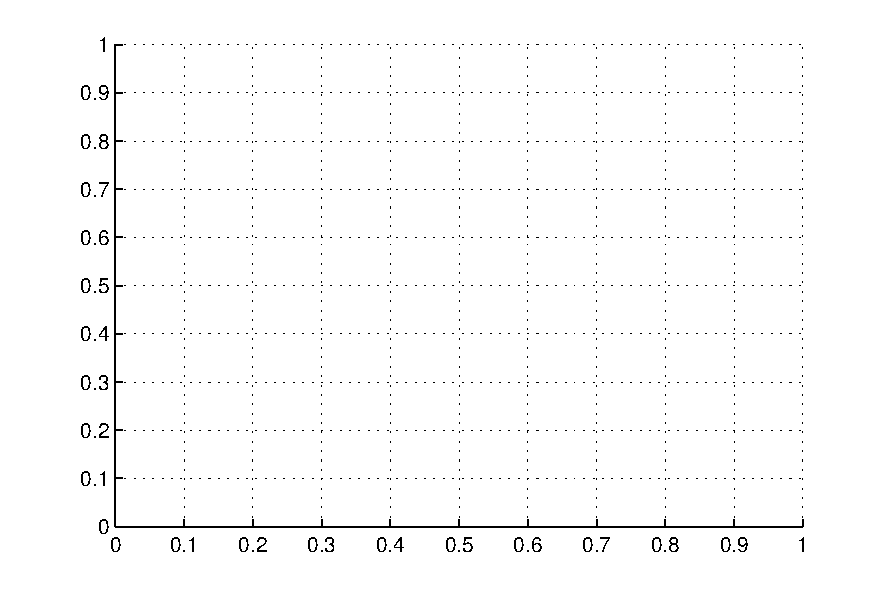
\includegraphics[scale=0.5]{emptiness.pdf}
\caption{This is emptiness, it earns no points.}
\end{center}
\end{figure}

\newproblem{3pt} 
Use \verb|conv2| between log of $\theta$ and each sequence $\xx$ to efficiently compute posterior.
Note that \verb|conv2| flips one of its inputs.

\begin{verbatim}
function [q,ll] = estep2(theta,X)
A = size(theta,1); % size of alphabet
L = size(theta,2); % length of motif
N = size(X,2);     % length of full sequence
T = size(X,3);     % number of examples
q = zeros(N-L+1,T);
ll = 0;
for t=1:T
    xt = X(:,:,t);
    ... use conv2 ...
    lp = logsum(q(...));
    ll = ll + lp;
    q(...) = exp(q(...) - lp);
end

function l = logsum(v)
m = max(v); v = v - m;
l = log(sum(exp(v))) + m;
\end{verbatim}

Compare outputs of \verb|estep| and \verb|estep2| and make sure that they are, up to numerical error, the same.

Demonstrate speed-up for different N and L.

\end{document}
